\documentclass{article}


% if you need to pass options to natbib, use, e.g.:
%     \PassOptionsToPackage{numbers, compress}{natbib}
% before loading neurips_2022


% ready for submission
\usepackage{neurips_2022}

% to compile a preprint version, e.g., for submission to arXiv, add add the
% [preprint] option:
%     \usepackage[preprint]{neurips_2022}


% to compile a camera-ready version, add the [final] option, e.g.:
%     \usepackage[final]{neurips_2022}


% to avoid loading the natbib package, add option nonatbib:
%    \usepackage[nonatbib]{neurips_2022}

\usepackage{natbib}

\usepackage{times} 
\usepackage{helvet}  
\usepackage{courier}  
\usepackage{url}  
\usepackage{graphicx} 

\usepackage{amssymb}
\usepackage{amsthm}
\usepackage{amsmath}
\usepackage{algorithm}
\usepackage[noend]{algpseudocode}


\usepackage{multirow}
\usepackage{ctable}
\usepackage{color}
\usepackage{natbib}
\usepackage[normalem]{ulem}
\usepackage{caption, subcaption}


%\usepackage[style=authoryear]{biblatex}



\usepackage[utf8]{inputenc} % allow utf-8 input
\usepackage[T1]{fontenc}    % use 8-bit T1 fonts
\usepackage{hyperref}       % hyperlinks
\usepackage{url}            % simple URL typesetting
\usepackage{booktabs}       % professional-quality tables
\usepackage{amsfonts}       % blackboard math symbols
\usepackage{nicefrac}       % compact symbols for 1/2, etc.
\usepackage{microtype}      % microtypography
\usepackage{xcolor}         % colors

\theoremstyle{definition}
\newtheorem{defn}{Definition}[section]
\newtheorem{theorem}{Theorem}[section]
\newtheorem{lemma}{Lemma}[section]
\newtheorem{hypothesis}{Hypothesis}[section]
\newtheorem{assumption}{Assumption}
\newcommand{\Expect}[2]{\mathbb{E}_{#1}\left [#2 \right ]}
\newcommand{\RM}[1]{\textcolor{magenta}{\{RM: #1\}}}
\newcommand{\LF}[1]{\textcolor{blue}{\{LF: #1\}}}



\title{Effective meta-adaptation based on data-dependent PAC-Bayes bounds}


% The \author macro works with any number of authors. There are two commands
% used to separate the names and addresses of multiple authors: \And and \AND.
%
% Using \And between authors leaves it to LaTeX to determine where to break the
% lines. Using \AND forces a line break at that point. So, if LaTeX puts 3 of 4
% authors names on the first line, and the last on the second line, try using
% \AND instead of \And before the third author name.


\author{%
	Lior Friedman, Ron Meir \\
	The Viterbi Faculty of Electrical and Computer Engineering\\
	Technion - Israel Institute of Technology\\
	Haifa 3200003, Israel\\
	\texttt{\{liorf@campus,rmeir@ee\}.technion.ac.il} \\
}


\begin{document}
	
\maketitle

	\begin{abstract}
	\LF{Very rough draft, rewrite after finishing the rest of the paper}
	
	Over the last few years, the paradigm of meta-learning, or learning to learn, has been shown to be an effective way to solve several machine learning problems, with especially impressive empirical results for few-shot classification problems - an important setting to many real-world applications such as medical imaging and natural language processing.
		
	In an effort to understand and quantify the generalization capabilities of such methods, there have been several extensions of PAC-Bayes approaches and mutual-information bounds to the problem of meta-learning. While these extensions provide meaningful bounds and practical optimization methods, the focus of such analysis was always the meta-learning process. 
	
	As several recent works on PAC-Bayes bounds have shown, data-dependent bounds can lead to significantly tighter confidence intervals, and so it stands to reason that applying such bounds to the meta-testing process can provide us with meaningful risk certificates for few-shot classification.
	
	In this paper, we derive a novel data-dependent PAC-Bayes bound for meta-testing and demonstrate its efficacy for few-shot image classification. \LF{If time and results permit, also discuss forgetting here, ideally both theoretically and empirically}
		
	\end{abstract}


\section{Introduction}

\LF{TODO: start with a motivating example for meta-learning}

% ml, meta-learning and few-shot
Over the last few decades, the field of machine learning has developed rapidly both theoretically and as an engineering practice. Of particular interest is the task of learning and adapting quickly from only a few examples, and balancing prior experience and new information in order to solve new tasks effectively without overfitting.
One common approach to tackle this few-shot learning problem is that of meta-learning (or learning to learn), where training data is used to create a prior conducive to the downstream task. This approach has shown promising empirical results in a variety of domains (see survey \citep{Hospedales2021}), especially for cases with few test examples.

\LF{Need to mention the basic idea of meta-learning a distribution over priors for the test task}

In order to better understand the generalization capabilities of classification methods and give upper bounds on the gap between the training and test performance, several theoretical frameworks were devised.  Among these frameworks, methods based on PAC-Bayes bounds \citep{Mcallester} are of particular interest, as they result in practical optimization algorithms with potentially non-vacuous generalization guarantees with high probability. As such, it is not surprising that several works have extended the PAC-Bayes framework to the domain of meta-learning, such as \citet{Pentina2014}, \citet{Amit2018} and \citet{Rothfuss2020}.

There have been several recent works that showed non-vacuous generalization bounds for practical deep learning problems, such as the methods suggested by \citet{Dziugaite2017} and later improved by \citet{Perez-Ortiz2021}. In both cases, the use of a data-dependent prior was shown to be a major component in achieving these impressive results. As such, data-dependent PAC-Bayes bounds such as those proposed in \citet{Rivasplata2020} may be of great interest for meta-learning problems.

\LF{It may be a good idea to add a paragraph here about issues with meta-learning PB bounds and why data-dependent bounds can help - the benefit in meta-learning would be reducing the hyper-KL term, but usually the task-KL is a bigger issue there.}

In this paper, we utilize data-dependent PAC-Bayes bounds to provide an upper bound on the generalization error for meta-testing by adapting an existing distribution over priors to better fit the given test task. This approach allows us to use existing methods to meta-learn a distribution over training tasks and provides a potentially tighter guarantee for the new task, at the cost of partially forgetting the training tasks. 
We then use these bounds to develop a practical algorithm for meta-testing and adaptation.
Our main contributions are as follows: (i) A novel bound for adaptation in meta-learning using data-dependent priors (ii) A generic algorithm for meta-testing (iii) Empirical demonstration of the benefit of this method compared to standard meta-testing methods for few-shot image classification.

\LF{This is a poor intro, rework this later}

\section{Background} %also previous work?

\subsection{PAC-Bayes bounds}

The common setting for learning consists of a set of independent examples $S=\{z_i\}_{i=1}^{m}\subset \mathcal{Z}^m$, drawn from an unknown distribution $z_i\sim \mathcal{D}$. We denote $S\sim \mathcal{D}^m$ the distribution over the samples. Given a set of hypotheses $\mathcal{H}$ and a sample $S$, we would like to find a hypothesis $h\in \mathcal{H}$ that minimizes the \emph{expected loss} $\Expect{z\sim D}{l(h,z)}$, where $l:\mathcal{Z}\rightarrow [a,b]$ is a bounded\footnote{It is also possible to use unbounded loss functions with some concentration property such as a a sub-gamma distribution.} loss function.
Since $\mathcal{D}$ is unknown, the training data $S$ must be used to do so. 

The PAC-Bayes framework, first formulated by \citet{Mcallester}, takes as input the training data $S$ as well as an inductive bias in the form of a prior distribution $P$ over $\mathcal{H}$. These are then used to construct a posterior distribution $Q$ over $\mathcal{H}$, and $h\sim Q$ is then sampled.

More formally, we define the expected error $\mathcal{L}(h, D)\triangleq \Expect{z\sim D}{l(h,z)}$ and the empirical error $\hat{\mathcal{L}}(h, S)\triangleq \frac{1}{m}\sum_{i=1}^{m} l(h,z_i)$, and since in the PAC-Bayes setting we have a distribution $Q\in \mathcal{M}(\mathcal{H})$, we need to average these quantities over the posterior distribution:
$$\mathcal{L}(Q, D)\triangleq \Expect{h\sim Q}{\Expect{z\sim D}{l(h,z)}}, \hat{\mathcal{L}}(Q, S)\triangleq \Expect{h\sim Q}{\frac{1}{m}\sum_{i=1}^{m} l(h,z_i)}$$.

Following these definitions, we can derive a PAC-Bayes theorem for the single task setting, as formulated by \citet{Mcallester}:

\begin{theorem} (McAllister's single task bound) \label{thm:classic-pb}
	Let $P\in \mathcal{M}(\mathcal{H})$ be some prior distribution over $\mathcal{H}$.
	For any $\delta \in (0,1)$, the following inequality holds uniformly for all posteriors $Q\in \mathcal{M}(\mathcal{H})$ with probability at least $1-\delta$ over the choice of $S$:
	
	$$\mathcal{L}(Q, D) \leq \hat{\mathcal{L}}(Q, S)+\sqrt{\frac{D_{KL}(Q||P)+log\frac{m}{\delta}}{2(m-1)}}$$
	
	Where $D_{KL}(Q||P)\triangleq \Expect{h\sim Q}{log\frac{Q(h)}{P(h)}}$ is the Kullback-Leibler divergence.
\end{theorem}

This theorem is commonly interpreted as the expected error being upper bounded by the empirical error plus a complexity term that depends on the probability, the sample size, and the divergence of the posterior from the prior. Since this theorem holds uniformly over all $Q$, we can derive a practical learning algorithm that chooses $Q$ such that it minimizes the right-hand-side of this bound. Naturally, this bound is affected by the choice of $P$, as ideally we would like to have a prior that is close to posteriors that achieve low empirical error, thereby motivating the notion of data-dependent priors.

\subsection{Data-dependent priors}

It is quite clear from the bound presented in Theorem \ref{thm:classic-pb} that if we knew in advance a posterior distribution $Q_S$ that minimizes $\hat{\mathcal{L}}(Q_S, S)$, then picking a prior $P=Q_S$ would give us an optimal upper bound on the expected error $\mathcal{L}(Q, D)$.
Classical PAC-Bayes bound, however, assume that $P$ must be picked independently of the sample $S$, often resulting in the complexity term $D_{KL}(Q||P)$ to be a dominant part of the bound, which may render it vacuous. 

While it is theoretically possible to pick the prior $P$ based on the true data distribution $\mathcal{D}$, the PAC-Bayes framework assumes this distribution is unknown, and therefore it cannot be used directly. In order to pick a better prior based on $S$, previous methods have relied on differential privacy \citep{Dziugaite2018} as a proxy to stability that allows the use of $S$ in estimating the prior. Another promising alternative method that was shown to be effective \citep{Dziugaite2017, Perez-Ortiz2021} was to split the training data into a prior estimation set and a bound optimization set. Since these sets do not overlap and the sample $S$ is assumed to be i.i.d., this approach has resulted in data-dependent priors that also give much tighter upper bounds on the expected error for neural networks compared to traditional data-free priors and PAC-Bayes bounds.

Both of these solutions have been shown to provide meaningful, non-vacuous generalization bounds as well as high test accuracy for classification problems with a sufficiently large training set. For few-shot learning problems, however, these approaches by themselves are unlikely to be sufficient. For this reason, a meta-learned prior may provide an elegant solution.

\subsection{PAC-Bayes bounds for meta-learning}

In the meta-learning setting, we are given as input several training tasks from a single task environment. A meta-learning algorithm must extract the necessary common knowledge (in the form of a prior) to efficiently learn new tasks in the same environment. Following the formulation of PAC-Bayes bounds for lifelong learning \citep{Pentina2014} and meta-learning \citep{Amit2018}, we assume a shared sample space $\mathcal{Z}$, hypothesis space $\mathcal{H}$ and loss function $l:\mathcal{Z}\times \mathcal{H}\rightarrow [a,b]$, and a set of training datasets $\{S_1,...,S_N\}$ of size $m$ each\footnote{Training datasets may differ in size, but we assume equal sizes for convenience.}. Each training dataset $S_i$ is assumed to come from an unknown distribution $S_i\sim \mathcal{D}_i$, and these distributions are sampled i.i.d. from a shared (and also unknown) task distribution $D_i\sim \tau$.

The goal of a meta-learning algorithm is to construct a prior $P$ such that given samples $S_T$ from a new task $\mathcal{D}_T\sim \tau$, the base learner uses both to construct a posterior $Q(P, S_T)$ over the hypothesis space $\mathcal{H}$. In order to evaluate our constructed prior, we can consider its expected error:

$$\mathcal{L}(P, \tau)\triangleq \Expect{D\sim \tau}{\Expect{S\sim D^m}{\Expect{h\sim Q(P, S)}{\mathcal{L}(h, D)}}}$$

The meta-learning PAC-Bayes framework can thus be seen as learning a hyper-posterior distribution $\mathcal{Q}\in \mathcal{M}(\mathcal{M}(\mathcal{H}))$ over priors. Similarly to the single task setting, we assume access to a hyper-prior distribution $\mathcal{P}\in \mathcal{M}(\mathcal{M}(\mathcal{H}))$, as well as training datasets $\{S_1,...,S_N\}$.
We would like to optimize over $\mathcal{Q}$ in order to minimize the expected transfer error $\mathcal{L}(\mathcal{Q}, \tau) \triangleq \Expect{P\sim \mathcal{Q}}{\mathcal{L}(P, \tau)}$.
Since the true task distribution $\tau$ is unknown, we can use an estimate in the form of the empirical multi-task error $$\hat{\mathcal{L}}(\mathcal{Q}, S_1,...,S_N)\triangleq \Expect{P\sim \mathcal{H}}{\frac{1}{N}\sum_{i=1}^{N}\hat{\mathcal{L}}(Q(P, S_i), S_i)}$$. A similar approach to the single task case leads us to PAC-Bayes bounds on the transfer error, such as the following:

\begin{theorem} (Meta-learning bound \citep{Amit2018}) \label{thm:meta-pb}
	Let $\mathcal{P}\in \mathcal{M}(\mathcal{M}(\mathcal{H}))$ be some hyper-prior distribution, and let $Q: \mathcal{Z}^m\times\mathcal{M}(\mathcal{H})\rightarrow \mathcal{M}(\mathcal{H})$ be a given base learner.
	For any $\delta \in (0,1)$, the following inequality holds uniformly for all hyper-posteriors $\mathcal{Q}\in \mathcal{M}(\mathcal{M}(\mathcal{H}))$ with probability at least $1-\delta$ over the choice of $D_1,...,D_N\sim \tau, S_i\sim D_i$:
	
	\begin{align} \label{eq:meta-pb-amit}
	\begin{split}
	\mathcal{L}(\mathcal{Q}, \tau) &\leq \hat{\mathcal{L}}(\mathcal{Q}, S_1,...,S_N) \\
	&+\sqrt{\frac{D_{KL}(\mathcal{Q}||\mathcal{P})+log\frac{2N}{\delta}}{2(N-1)}} \\
	&+\frac{1}{N}\sum_{i=1}^{N}\sqrt{\frac{D_{KL}(\mathcal{Q}||\mathcal{P})+\Expect{P\sim \mathcal{Q}}{D_{KL}(Q(P,S_i)||P)}+log\frac{2Nm}{\delta}}{2(m-1)}}
	\end{split}
	\end{align}

\end{theorem}

This bound on the transfer error contains two complexity terms: an environment-level complexity term that decreases as $N\rightarrow \infty$, and a second task-level term that decreases as $m\rightarrow \infty$. A potentially tighter and simpler version of this bound was recently proposed by \cite{Rothfuss2020}, which notably also contains two such complexity terms.

An important technique used in the derivation of these bounds is the definition of a 2-level prior $(\mathcal{P}, P^N)=\mathcal{P}\times \prod_{i=1}^{N}P$ as the distribtuion in which we first sample $P\sim \mathcal{P}$ and then use it as the posterior for all tasks. Similarly, the 2-level posterior is defined as $(\mathcal{Q}, Q^N)=\mathcal{Q}\times \prod_{i=1}^{N}Q(P, S_i)$. These definitions are then used alongside known PAC-Bayes bounds to provide a bound on the transfer error. Given these definitions, the KL-divergence $D_{KL}\left ((\mathcal{Q}, Q^N)||(\mathcal{P}, P^N)\right )$ can be decomposed as:

\begin{equation} \label{eq:kl-decompose}
 D_{KL}\left ((\mathcal{Q}, Q^N)||(\mathcal{P}, P^N)\right ) = D_{KL}(\mathcal{Q}||\mathcal{P}) + \Expect{P\sim \mathcal{Q}}{\sum_{i=1}^{N}D_{KL}(Q(P, S_i)||P)}
\end{equation}

\section{Meta-adaptation for meta-testing}

As we have seen, the meta-learning framework provides us with an informative hyper-posterior from which a good prior (i.e. one with low expected error) can be sampled. It is possible to use algorithms for learning data-dependent priors given a sampled prior $P\sim \mathcal{Q}$, but although empirical performance of meta-learning methods suggest that this is effective, doing so does not provide a better risk certificate compared to using a random, data-free prior. 

In this section, we will introduce a PAC-Bayes bound for meta-adaptation of a given hyper-posterior to the provided test set that can potentially provide us with tighter risk certificates given an informative hyper-posterior distribution.
In order to do so, we will make use of an existing PAC-Bayes inequality \citep{Rivasplata2020} for stochastic kernels that allow for data-dependent priors, restricted to our setting:

\begin{theorem} (PAC-Bayes for stochastic kernels - adapted from Theorem 2 in \citet{Rivasplata2020}) \label{thm:rivasplata-pb}
	Let $P\in \mathcal{K}(\mathcal{Z}^m, \mathcal{H})$ be a stochastic kernel, let $A: \mathcal{Z}^m\times \mathcal{H}\rightarrow \mathbb{R}^k$ be a measurable function for some positive integer $k$ and $F:\mathbb{R}^k\rightarrow \mathbb{R}$ be a convex function.
	Define $f\triangleq F\circ A$, and let 
	$$\xi=\int_{\mathcal{Z}^m}\int_{\mathcal{H}}e^{f(S, h)}P_S(dh)\mathcal{D}(dS)$$
	Such that $P_S$ is the distribution over $\mathcal{H}$ corresponding to the sampled $S$.
	
	Assuming $\xi$ is finite, for any $\delta \in (0,1)$, the following inequality holds uniformly for all posteriors $Q\in \mathcal{K}(\mathcal{Z}^m, \mathcal{H})$ with probability at least $1-\delta$ over the choice of $S\sim \mathcal{D}$:
	
	\begin{equation} \label{eq:ribasplata-pb}
	\Expect{h\sim Q_S}{f(S, h)} \leq D_{KL}(Q_S||P_S)+log\left (\frac{\xi}{\delta}\right )
	\end{equation}
\end{theorem}

This theorem provides a general PAC-Bayes bound that can be easily applied to data-dependent priors through the exponential moment term $\xi$. One particularly appealing application of this general bound is for data-dependent Gibbs priors, as they conform to algorithmic stability properties \citep{Kuzborskij2019} and therefore have a bounded moment term.

\begin{defn} \label{defn:Gibbs}
	The Gibbs distribution with parameter $\beta>0$ is defined as $$Q(P,S)(h)=\frac{P(h)e^{-\beta \hat{\mathcal{L}}(h,S)}}{Z_\beta(S,P)}$$ 
	where 
	$$Z_\beta(S,P)=\Expect{h\sim P}{e^{-\beta\hat{\mathcal{L}}(h,S)}}$$
\end{defn}

Let $\mathcal{Q}_{1:N}$ be a hyper-posterior learned on the training data $\{S_1,...,S_N\}$, and let $$\mathcal{Q}_{1:N,T}= \frac{\mathcal{Q}_{1:N}e^{-\gamma\hat{\mathcal{L}}(P,S_T)}}{Z_\gamma(S_T, \mathcal{Q}_{1:N})}$$ be the Gibbs posterior for the meta-learned problem with meta-normalization term $$Z_\gamma(S_T, \mathcal{Q}_{1:N})=\Expect{P\sim \mathcal{Q}_{1:N}}{e^{-\gamma\hat{\mathcal{L}}(P,S_T)}}$$.

\LF{Using the base learner $Q(P,S_T)$ here would change the $L_{meta}$ term to $L_{full}$}

Using Theorem \ref{thm:rivasplata-pb} with a 2-level hypothesis $(\mathcal{Q},Q), (\mathcal{Q}_{1:N}, P)$, where we denote $Q=Q(P, S_T)$ for brevity, by choosing $f(\mathcal{Q}, Q, S_T)\triangleq\lambda\left (\mathcal{L}(\mathcal{Q}, D_T)-\hat{\mathcal{L}}(\mathcal{Q}, S_T)\right )$, we get with probability at least $1-\delta_T$ over the draw of $S_T$ that:

$$\Expect{P\sim \mathcal{Q}_{1:N,T},h\sim Q(P,S_T)}{\lambda\left (\mathcal{L}(h, D_T)-\hat{\mathcal{L}}(h, S_T)\right )} \leq D_{KL} \Big (((\mathcal{Q}_{1:N,T}, Q(P,S_T))||(\mathcal{Q}_{1:N}, P) \Big )+ ln\frac{\xi(\lambda,\mathcal{Q}_{1:N})}{\delta_T}$$

where $$\xi(\lambda,\mathcal{Q}_{1:N})=\Expect{S\sim D_T, P\sim \mathcal{Q}_{1:N}, h\sim P}{e^{\lambda\left (\mathcal{L}(h, D_T)-\hat{\mathcal{L}}(h, S_T)\right )}}$$

We note that $\xi(\lambda,\mathcal{Q}_{1:N})$ may or may not depend on $S_T$. \LF{Interesting idea: can use $(\mathcal{Q}_{1:N}, Q)$ as prior, so we only adapt the hyper distribution. This would remove the base learner KL term, and since we use Gibbs posteriors the moment is bounded.} Using the product property of the KL-divergence (as in Equation \ref{eq:kl-decompose}), we can write this inequality as:

$$\mathcal{L}(\mathcal{Q}_{1:N,T}, D_T) \leq \hat{\mathcal{L}}(\mathcal{Q}_{1:N,T}, S_T) + \frac{1}{\lambda}D_{KL}(\mathcal{Q}_{1:N,T}||\mathcal{Q}_{1:N})+\frac{1}{\lambda}\Expect{P\sim \mathcal{Q}_{1:N,T}}{D_{KL}(Q(P,S_T)||P)}+\frac{1}{\lambda}ln\frac{\xi(\lambda,\mathcal{Q}_{1:N})}{\delta_T}$$


If we choose the base learner $Q$ to be the Gibbs learner with parameter $\beta$ (see Definition \ref{defn:Gibbs}), we have:

$$D_{KL}(Q(P,S_T)||P)=-\beta\hat{\mathcal{L}}(Q(P,S_T), S_T)-lnZ_\beta(S_T,P)$$

Where, as defined above, $$Z_\beta(S,P)=\Expect{h\sim P}{e^{-\beta\hat{\mathcal{L}}(h,S)}}$$

And therefore,

$$\mathcal{L}(\mathcal{Q}_{1:N,T}, D_T) \leq (1-\frac{\beta}{\lambda})\hat{\mathcal{L}}(\mathcal{Q}_{1:N,T}, S_T) + \frac{1}{\lambda}D_{KL}(\mathcal{Q}_{1:N,T}||\mathcal{Q}_{1:N})-\frac{1}{\lambda}\Expect{P\sim \mathcal{Q}_{1:N,T}}{lnZ_{\beta}(S_T,P)}+\frac{1}{\lambda}ln\frac{\xi(\lambda,\mathcal{Q}_{1:N})}{\delta_T}$$

Since our hyper-posterior is also a Gibbs distribution, we have 
$$KL(\mathcal{Q}_{1:N,T}||\mathcal{Q}_{1:N})=
-\gamma\hat{\mathcal{L}}'(\mathcal{Q}_{1:N,T}, S_T)-ln\Expect{P\sim \mathcal{Q}_{1:N}}{e^{-\gamma\hat{\mathcal{L}}(P,S_T)}}$$ 

Where $\hat{\mathcal{L}}'(\mathcal{Q},S)=\mathbb{E}_{P\sim \mathcal{Q}}\mathbb{E}_{h\sim P}\left [\hat{\mathcal{L}}(h, S)\right ]$ is the average empirical loss without prior adaptation.
So,
\begin{align*} 
\begin{split}
\mathcal{L}(\mathcal{Q}_{1:N,T}, D_T) \leq &(1-\frac{\beta}{\lambda})\hat{\mathcal{L}}(\mathcal{Q}_{1:N,T}, S_T) -\frac{\gamma}{\lambda}\hat{\mathcal{L}}'(\mathcal{Q}_{1:N,T}, S_T) \\ &- \frac{1}{\lambda}ln\Expect{P\sim \mathcal{Q}_{1:N}}{e^{-\gamma\hat{\mathcal{L}}(P,S_T)}}-\frac{1}{\lambda}\Expect{P\sim \mathcal{Q}_{1:N,T}}{lnZ_{\beta}(S_T,P)}\\ &+\frac{1}{\lambda}ln\frac{\xi(\lambda,\mathcal{Q}_{1:N})}{\delta_T}
\end{split}
\end{align*}


\begin{figure}
	\centering
	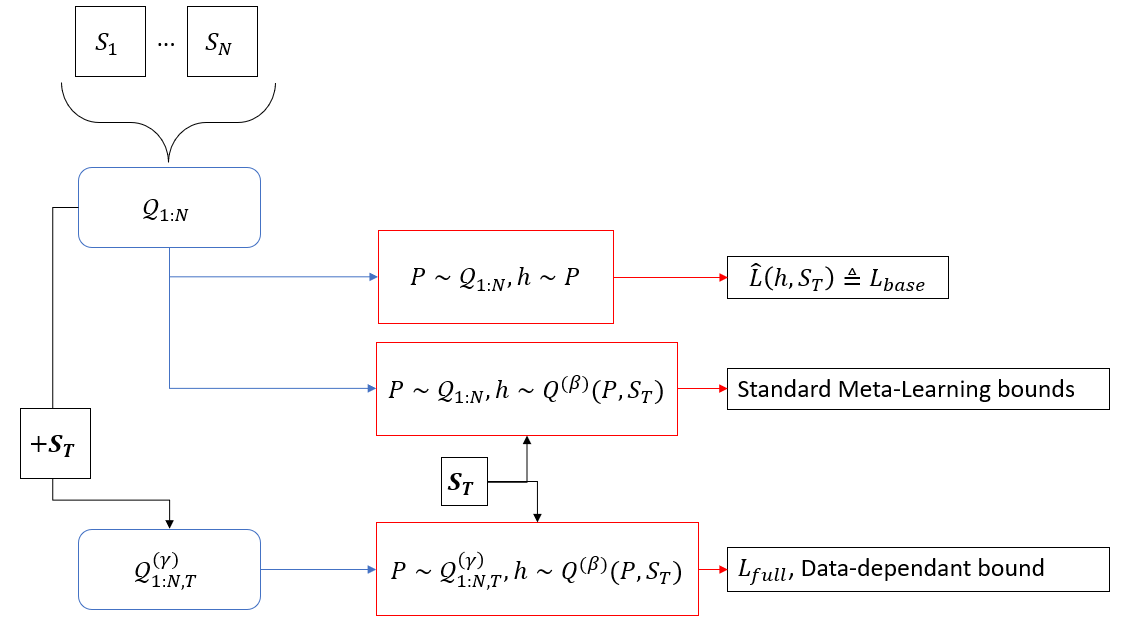
\includegraphics[width=0.9\textwidth]{data_dependant_adaptation.PNG}
	\caption{Flowchart of hyper-posterior construction settings detailing how the test data $S_T$ can be used. A hyper-prior $\mathcal{Q}_{1:n}$ is learned from the training data. This hyper-prior can be sampled and then a hypothesis can be sampled from the resulting prior, thereby ignoring the test data. Standard meta-learning bounds use the test data to adapt the sampled prior before sampling a specific hypothesis. Our approach using data-dependent bounds also applies $S_T$ to the hyper-prior, resulting in a data-dependent hyper-posterior $\mathcal{Q}_{1:n, T}$. }
	\label{fig:data_dependant_bound}
\end{figure}

In order to clarify this expression, we will use more intuitive definitions for our empirical losses:
\begin{defn}
	We define $$\hat{\mathcal{L}}_{full}\triangleq \hat{\mathcal{L}}^{(\gamma,\beta)}(\mathcal{Q}_{1:N,T}, S_T)=\mathbb{E}_{P\sim \mathcal{Q}^{\gamma}_{1:N,T}}\mathbb{E}_{h\sim Q^{\beta}(P,S_T)}\left [\hat{\mathcal{L}}(h, S_T)\right ]$$ as the fully adapted loss, meaning $S_T$ is used to adapt both the hyper-prior ($\mathcal{Q}_{1:N}$) and the sampled prior. $\hat{\mathcal{L}}_{full}$ is a function of both $\gamma$ and $\beta$.
	
	We define $$\hat{\mathcal{L}}_{meta}\triangleq \hat{\mathcal{L}}'^{(\gamma)}(\mathcal{Q}_{1:N,T}, S_T)=\mathbb{E}_{P\sim \mathcal{Q}^{\gamma}_{1:N,T}}\mathbb{E}_{h\sim P}\left [\hat{\mathcal{L}}(h, S_T)\right ]$$ 
	as the meta-adapted loss, meaning $S_T$ is used only on the hyper-prior level. $\hat{\mathcal{L}}_{meta}$ is a function of $\gamma$.
	
	We define $$\hat{\mathcal{L}}_{base}\triangleq \hat{\mathcal{L}}'(\mathcal{Q}_{1:N}, S_T)=\mathbb{E}_{P\sim \mathcal{Q}_{1:N}}\mathbb{E}_{h\sim P}\left [\hat{\mathcal{L}}(h, S_T)\right ]$$ as the base empirical loss on the hyper-prior. $\hat{\mathcal{L}}_{base}$ does not depend on $\gamma$ and $\beta$.
\end{defn}

Using these definitions, we get:

$$\mathcal{L}(\mathcal{Q}_{1:N,T}, D_T) \leq (1-\frac{\beta}{\lambda})\hat{\mathcal{L}}_{full} -\frac{\gamma}{\lambda}\hat{\mathcal{L}}_{meta} - \frac{1}{\lambda}lnE_{P\sim \mathcal{Q}_{1:N}}\left [e^{-\gamma\hat{\mathcal{L}}(P,S_T)}\right ]-\frac{1}{\lambda}E_{P\sim \mathcal{Q}_{1:N,T}}\left [lnZ_{\beta}(S_T,P)\right ]+\frac{1}{\lambda}ln\frac{\xi(\lambda,\mathcal{Q}_{1:N})}{\delta_T}$$

%We note that the second term is not quite the same as the third ($Z_\beta(S,P)=E_{h\sim P} \left [ e^{-\beta\hat{\mathcal{L}}(h,S)}\right ]$) as the order of expectations is different and the hyper-prior is also different. 

By simplifying the third and fourth terms using Jensen's inequality , we get:

\begin{equation} \label{eq:pb-adapt-multi}
\mathcal{L}(\mathcal{Q}_{1:N,T}, D_T) \leq 
(1-\frac{\beta}{\lambda})\hat{\mathcal{L}}_{full} +(\frac{\beta-\gamma}{\lambda})\hat{\mathcal{L}}_{meta} + \frac{\gamma}{\lambda}\hat{\mathcal{L}}_{base} 
+\frac{1}{\lambda}ln\frac{\xi(\lambda,\mathcal{Q}_{1:N})}{\delta_T}
\end{equation}

This equation gives us a generalization bound that considers the empirical loss of the hyper-prior as well as the empirical loss for the posterior, thereby giving us the following theorem:

\begin{theorem} \label{thm:main-result}
	Let $\mathcal{Q}_{1:N}$ be a hyper-posterior (e.g. the result of meta-training on $\{S_1,...,S_N\}$), and let $\mathcal{D}_T\sim \tau$ be a given test task. Let $$\mathcal{Q}_{1:N,T}= \frac{\mathcal{Q}_{1:N}e^{-\gamma\hat{\mathcal{L}}(P,S_T)}}{Z_\gamma(S_T, \mathcal{Q}_{1:N})}$$ be the empirical Gibbs distribution for given dataset $S_T\sim \mathcal{D}_T$.
	
	With probability at least $1-\delta_T$ over the draw of $S_T\sim \mathcal{D}_T$:
	
	$$\mathcal{L}(\mathcal{Q}_{1:N,T}, D_T) \leq 
	(1-\frac{\beta}{\lambda})\hat{\mathcal{L}}_{full} +(\frac{\beta-\gamma}{\lambda})\hat{\mathcal{L}}_{meta} + \frac{\gamma}{\lambda}\hat{\mathcal{L}}_{base} 
	+\frac{1}{\lambda}ln\frac{\xi(\lambda,\mathcal{Q}_{1:N})}{\delta_T}$$
\end{theorem}

\LF{Mention that we could have used other options for $f$ to get Seeger-style bounds or other such results? Using the same base-prior and posterior removes all terms with $\beta$ }

Theorem \ref{thm:main-result} provides an upper bound on the expected error for a given test task that depends on the empirical error of the base learner $\hat{\mathcal{L}}_{base}$ as well as the empirical loss of the newly constructed hyper-posterior $\mathcal{Q}_{1:N,T}$. Since the bound applies uniformly for all $\gamma>0,\beta>0,\lambda>0$, this bound can be further optimized by choosing optimal values for $\gamma, \beta, \lambda$. This can be done by deriving the right-hand-side of Equation \ref{eq:pb-adapt-multi} and comparing to zero. 

\subsection{Optimizing $\gamma$}

Deriving Equation \ref{eq:pb-adapt-multi} by $\gamma$ gets us:

\begin{equation} \label{eq:gamma-deriv}
(1-\frac{\beta}{\lambda})\frac{d}{d\gamma}\hat{\mathcal{L}}_{full} -\frac{1}{\lambda}\hat{\mathcal{L}}_{meta} + (\frac{\beta-\gamma}{\lambda})\frac{d}{d\gamma}\hat{\mathcal{L}}_{meta} +\frac{1}{\lambda}\hat{\mathcal{L}}_{base} =0
\end{equation}

We must calculate the derivatives of the expected losses: \LF{move to appendix?}

$$\frac{d}{d\gamma}\hat{\mathcal{L}}_{meta}=\int \frac{d}{d\gamma}\mathcal{Q}_{1:N,T}(P)\hat{\mathcal{L}}(P, S_T)dP=\int \mathcal{Q}_{1:N}(P)\hat{\mathcal{L}}(P, S_T)\frac{d}{d\gamma}
\frac{e^{-\gamma\hat{\mathcal{L}}(P,S_T)}}{\Expect{P\sim \mathcal{Q}_{1:N}}{e^{-\gamma\hat{\mathcal{L}}(P,S_T)}}}dP$$

$$=\int \mathcal{Q}_{1:N}(P)\hat{\mathcal{L}}(P, S_T)\frac{-\hat{\mathcal{L}}(P,S_T)e^{-\gamma\hat{\mathcal{L}}(P,S_T)}\Expect{P\sim \mathcal{Q}_{1:N}}{e^{-\gamma\hat{\mathcal{L}}(P,S_T)}}
-e^{-\gamma\hat{\mathcal{L}}(P,S_T)}\Expect{P\sim \mathcal{Q}_{1:N}}{-\hat{\mathcal{L}}(P,S_T)e^{-\gamma\hat{\mathcal{L}}(P,S_T)} }}{\Expect{P\sim \mathcal{Q}_{1:N}}{e^{-\gamma\hat{\mathcal{L}}(P,S_T)}}^2}dP$$


$$=\int \mathcal{Q}_{1:N,T}(P)\hat{\mathcal{L}}(P, S_T)\left (-\hat{\mathcal{L}}(P,S_T)-
\frac{\Expect{P\sim \mathcal{Q}_{1:N}}{-\hat{\mathcal{L}}(P,S_T)e^{-\gamma\hat{\mathcal{L}}(P,S_T)} }}{\Expect{P\sim \mathcal{Q}_{1:N}}{e^{-\gamma\hat{\mathcal{L}}(P,S_T)}}}\right)dP$$

To conclude our calculation of the derivative, we get:

$$\frac{d}{d\gamma}\hat{\mathcal{L}}_{meta}=-\Expect{P\sim \mathcal{Q}_{1:N,T}}{\hat{\mathcal{L}}(P,S_T)^2}-\frac{\Expect{P\sim \mathcal{Q}_{1:N}}{-\hat{\mathcal{L}}(P,S_T)e^{-\gamma\hat{\mathcal{L}}(P,S_T)} }}{\Expect{P\sim \mathcal{Q}_{1:N}}{e^{-\gamma\hat{\mathcal{L}}(P,S_T)}} }\hat{\mathcal{L}}_{meta} $$

Very similarly, since only the hyper-posterior $\mathcal{Q}_{1:N,T}$ is a 
function of $\gamma$, we have:

$$\frac{d}{d\gamma}\hat{\mathcal{L}}_{full}=-\Expect{P\sim \mathcal{Q}_{1:N,T}}{\hat{\mathcal{L}}(P,S_T)\hat{\mathcal{L}}\left (Q(P,S_T),S_T\right )}-\frac{\Expect{P\sim \mathcal{Q}_{1:N}}{-\hat{\mathcal{L}}(P,S_T)e^{-\gamma\hat{\mathcal{L}}(P,S_T)} }}{\Expect{P\sim \mathcal{Q}_{1:N}}{e^{-\gamma\hat{\mathcal{L}}(P,S_T)}} }\hat{\mathcal{L}}_{full} $$

Marking $R(\gamma)=\frac{\Expect{P\sim \mathcal{Q}_{1:N}}{-\hat{\mathcal{L}}(P,S_T)e^{-\gamma\hat{\mathcal{L}}(P,S_T)} }}{\Expect{P\sim \mathcal{Q}_{1:N}}{e^{-\gamma\hat{\mathcal{L}}(P,S_T)}} }$ for convenience, we use Equation \ref{eq:gamma-deriv} and replace the derivatives with this expression to find the optimal value of $\gamma$: 

\begin{align*} 
\begin{split}
&-(\lambda-\beta)\left (\Expect{P\sim \mathcal{Q}_{1:N,T}}{\hat{\mathcal{L}}(P,S_T)\hat{\mathcal{L}}\left (Q(P,S_T),S_T\right )}+R(\gamma)\hat{\mathcal{L}}_{full}\right )\\& - (\beta-\gamma)\left (\Expect{P\sim \mathcal{Q}_{1:N,T}}{\hat{\mathcal{L}}(P,S_T)^2}+R(\gamma)\hat{\mathcal{L}}_{meta}\right )\\& - \hat{\mathcal{L}}_{meta}+\hat{\mathcal{L}}_{base} = 0
\end{split}
\end{align*}

\begin{align*} 
\begin{split}
-(\beta-\gamma) = \frac{\hat{\mathcal{L}}_{meta}-\hat{\mathcal{L}}_{base}+(\lambda-\beta)
	\left (\Expect{P\sim \mathcal{Q}_{1:N,T}}{\hat{\mathcal{L}}(P,S_T)\hat{\mathcal{L}}(Q(P,S_T),S_T)}+R(\gamma)\hat{\mathcal{L}}_{full}\right )}{\Expect{P\sim \mathcal{Q}_{1:N,T}}{\hat{\mathcal{L}}(P,S_T)^2}+R(\gamma)\hat{\mathcal{L}}_{meta}}
\end{split}
\end{align*}

\begin{align} \label{eq:meta-pb-gamma}
\begin{split}
\gamma = \beta+\frac{\hat{\mathcal{L}}_{meta}-\hat{\mathcal{L}}_{base}+(\lambda-\beta)\left (\Expect{P\sim \mathcal{Q}_{1:N,T}}{\hat{\mathcal{L}}(P,S_T)\hat{\mathcal{L}}(Q(P,S_T),S_T)}+R(\gamma)\hat{\mathcal{L}}_{full}\right )}{\Expect{P\sim \mathcal{Q}_{1:N,T}}{\hat{\mathcal{L}}(P,S_T)^2}+R(\gamma)\hat{\mathcal{L}}_{meta}}
\end{split}\hfill
\end{align}

We note that this implicit function encourages an equilibrium for $\gamma$, as a negative value of $\hat{\mathcal{L}}_{meta}-\hat{\mathcal{L}}_{base}$ (meaning the meta-adaptation is beneficial) encourages lowering $\gamma$, and a negative value encourages increasing $\gamma$.

\subsection{Optimizing $\beta$}

Since neither $\hat{\mathcal{L}}_{meta}$ nor the moment $\xi$ depend on $\beta$, deriving Equation \ref{eq:pb-adapt-multi} by $\beta$ gives us:

$$-\hat{\mathcal{L}}_{full}+(\lambda-\beta)\frac{d}{d\beta}\hat{\mathcal{L}}_{full}+\hat{\mathcal{L}}_{meta}=0 $$

In a similar manner to before, we get

$$-(\lambda-\beta)\mathbb{E}_{P\sim \mathcal{Q}_{1:N,T}}\Expect{h\sim Q(P,S_T)}{\hat{\mathcal{L}}(h,S_T)^2+R'(\beta)\hat{\mathcal{L}}(h, S_T) } =\hat{\mathcal{L}}_{full}-\hat{\mathcal{L}}_{meta} $$

Where $R'(\beta)=\frac{\Expect{h\sim P}{-\hat{\mathcal{L}}(h,S_T)e^{-\beta\hat{\mathcal{L}}(h,S_T)} }}{\Expect{h\sim P}{e^{-\beta\hat{\mathcal{L}}(h,S_T)} }}$

And so we get for $\beta$:

\begin{align} \label{eq:meta-pb-beta}
\begin{split}
\beta = \lambda+\frac{\hat{\mathcal{L}}_{full}-\hat{\mathcal{L}}_{meta}}{\mathbb{E}_{P\sim \mathcal{Q}_{1:N,T}}\Expect{h\sim Q(P,S_T)}{\hat{\mathcal{L}}(h,S_T)^2+R'(\beta)\hat{\mathcal{L}}(h, S_T) }}
\end{split}
\end{align}

We note that the denominator is positive, so this is an implicit function of $\beta$ where it decreases proportionally to the prediction gain from the base learner  $\hat{\mathcal{L}}_{full}-\hat{\mathcal{L}}_{meta}$. Similarly to Equation \ref{eq:meta-pb-gamma}, this encourages an equilibrium value for $\beta$.

\subsection{Optimizing $\lambda$}

Finally, deriving Equation \ref{eq:pb-adapt-multi} by $\lambda$ gets us:

$$\frac{\beta}{\lambda^2} \hat{\mathcal{L}}_{full}-\frac{\beta-\gamma}{\lambda^2}\hat{\mathcal{L}}_{meta}-\frac{\gamma}{\lambda^2}\hat{\mathcal{L}}_{base}-\frac{1}{\lambda^2}ln\frac{\xi(\mathcal{Q}_{1:N}\lambda)}{\delta_T}+\frac{1}{\lambda}\frac{d}{d\lambda}ln\xi(\mathcal{Q}_{1:N},\lambda)=0$$

Multiplying by $\lambda^2$ gives:

$$\beta \hat{\mathcal{L}}_{full}-(\beta-\gamma)\hat{\mathcal{L}}_{meta}-\gamma\hat{\mathcal{L}}_{base}-ln\frac{\xi(\mathcal{Q}_{1:N}\lambda)}{\delta_T}+\lambda\frac{d}{d\lambda}ln\xi(\mathcal{Q}_{1:N},\lambda)=0$$

$$\beta(\hat{\mathcal{L}}_{full}-\hat{\mathcal{L}}_{meta})+\gamma(\hat{\mathcal{L}}_{meta}-\hat{\mathcal{L}}_{base})-ln\frac{\xi(\mathcal{Q}_{1:N}\lambda)}{\delta_T}+\lambda\frac{d}{d\lambda}ln\xi(\mathcal{Q}_{1:N},\lambda)=0$$

Since 
$$\frac{d}{d\lambda}ln\xi(\mathcal{Q}_{1:N},\lambda)=\frac{\mathbb{E}_{P\sim \mathcal{Q}_{1:N},S\sim D}\Expect{h\sim P}{(\mathbb{E}_S\hat{L}(h, S)-\hat{L}(h, S))e^{\lambda(\mathbb{E}_S\hat{L}(h, S)-\hat{L}(h, S))} }}{\mathbb{E}_{P\sim \mathcal{Q}_{1:N},S\sim D}\Expect{h\sim P}{e^{\lambda(E_S\hat{L}(h, S)-\hat{L}(h, S)} }}\triangleq R_\xi(\lambda)$$

We can write the above equation as:

$$\beta(\hat{\mathcal{L}}_{full}-\hat{\mathcal{L}}_{meta})+\gamma(\hat{\mathcal{L}}_{meta}-\hat{\mathcal{L}}_{base})-ln\frac{\xi(\mathcal{Q}_{1:N},\lambda)}{\delta_T}=-\lambda R_\xi(\lambda)$$

meaning,

\begin{align} \label{eq:meta-pb-lambda}
\begin{split}
\lambda = \frac{\beta(\hat{\mathcal{L}}_{meta}-\hat{\mathcal{L}}_{full})+\gamma(\hat{\mathcal{L}}_{base}-\hat{\mathcal{L}}_{meta})+ln\frac{\xi(\mathcal{Q}_{1:N},\lambda)}{\delta_T}}{R_\xi(\lambda)}
\end{split}
\end{align}

The first two terms of the numerator serve encourage an equilibrium for $\lambda$, since a positive prediction gain from the base learner $\hat{\mathcal{L}}_{full}-\hat{\mathcal{L}}_{meta}$ or a positive prediction gain from the meta-learner $\hat{\mathcal{L}}_{meta}-\hat{\mathcal{L}}_{base}$ both encourage a lower value for $\lambda$. The moment term $\xi(\mathcal{Q}_{1:N}, \lambda)$ increases with $\lambda$, so choosing a very large value for it may cause the moment to diverge and therefore violate the base conditions for the data-dependent (Theorem \ref{thm:rivasplata-pb}).

\section{Practical implementation and empirical evaluation}

As is usually the case with PAC-Bayes bounds, Theorem \ref{thm:main-result} provides us with a practical algorithm for meta-adaptation. In order to perform approximate posterior sampling for a Gibbs posterior, the SGLD (Stochastic Gradient Langevin Dynamics) algorithm \citep{Welling2011} can be used, assuming a sufficient number of iterations.
Combined with Monte-Carlo sampling to estimate expectations over priors, 
this approximation allows for the derivation of a complete practical algorithm for approximating $\mathcal{Q}_{1:N,T}$, which we describe in Algorithm \ref{alg1}.

\begin{algorithm}[H]
	\caption{Meta-adaptation and meta-testing}
	\label{alg1}
	\small
	\begin{algorithmic}
		\Function{Meta-adapt}{$\mathcal{Q}_{1:N}$, $S_T\sim \mathcal{D}_T$, $\lambda_T$}
		\State Initialize $\gamma, \beta, \lambda$ to some initial value 
		\State Initialize $\hat{\mathcal{Q}}_{1:N, T}\leftarrow \mathcal{Q}_{1:N}$
		\State Estimate $\hat{\mathcal{L}}_{base}$
		\While {$\gamma, \beta, \lambda$ not converged}
			\State gradients $\leftarrow \emptyset$
			\For {each Monte-Carlo estimation}
				\State Sample $P\sim \hat{\mathcal{Q}}_{1:N, T}$
				\State $h\leftarrow$ \Call{SGLD}{$P$, $S_T$, $\beta$} \Comment Approximate posterior sampling
				\State add $\nabla \hat{\mathcal{L}}(h, S_T)$ to gradients
			\EndFor
			\State $\nabla \hat{\mathcal{L}}(P, S_T)=$average(gradients)
			\State $\hat{\mathcal{Q}}_{1:N, T}\leftarrow$ \Call{SGLD-step}{$\hat{\mathcal{Q}}_{1:N, T}$, $\gamma$, $\nabla \hat{\mathcal{L}}(P, S_T)$} \Comment Update hyper-posterior
			
			\State Estimate $\hat{\mathcal{L}}_{full}, \hat{\mathcal{L}}_{meta}$
			\State Update $\gamma$ using Equation \ref{eq:meta-pb-gamma}
			\State Update $\beta$ using Equation \ref{eq:meta-pb-beta}
			\State Update $\lambda$ using Equation \ref{eq:meta-pb-lambda}
			
		\EndWhile
		\State \Return $\hat{\mathcal{Q}}_{1:N, T}, \beta$
		\EndFunction
		
		\Function{Meta-test}{$\mathcal{Q}_{1:N,T}$, $S_T\sim \mathcal{D}_T$, $\beta$} 
		\State Sample $P\sim \hat{\mathcal{Q}}_{1:N, T}$
		\State $h\leftarrow$ \Call{SGLD}{$P$, $S_T$, $\beta$} \Comment Sampling $h\sim P$ and using SGD is also valid
		\State Estimate test accuracy $\mathcal{L}_{01}(h, \mathcal{D}_T)$ using held-out test set
		\State \Return accuracy
		\EndFunction
	\end{algorithmic}
\end{algorithm}

We note that choosing $\gamma=\lambda=\sqrt{N}, \beta=\sqrt{m}$ may be a good initialization that ensures that for a data-free prior, the moment term $\xi$ does not diverge (with high probability), but other initializations may lead to faster convergence. Since estimating the optimal values for $\beta,\gamma,\lambda$ is both computationally expensive and may suffer from high variance in the few-shot classification setting, we consider a simpler variation of this algorithm by setting $\gamma, \beta, \lambda$ as hyper-parameters. This choice leads to a sub-optimal output, but still results in a valid hyper-posterior that can be evaluated and compared to standard meta-testing approaches.

\LF{Future extension: $\beta,\gamma,\lambda$ change during adaptation}

In order to demonstrate the efficacy of our meta-adaptation algorithm, we compare our approach to standard meta-testing for few-shot image classification tasks. The hypothesis space in question is a set of neural networks with a given architecture $\{h_w|w\in \mathbb{R}^d\}$. We use the cross-entropy loss during adaptation, despite the fact that it is not bounded. We note that a clipped variation of this loss does exist and conforms to theoretical guarantees, and in practice the cross-entropy loss tends to be low.

We conduct experiments on a task environment based on the MNIST dataset \citep{LeCun1998}, where each task was created by performing a random permutation on some of the image pixels. The number of pixels to be permuted and the total number of classes (referred to as ``ways'') was chosen in advance. We meta-learn a hyper-prior by running MAML \citep{Finn2017} for 100 meta-training iterations on randomly sampled training tasks, with 10 examples from each class. The resulting network weights were then used as the mean of a d-dimensional Gaussian (with variance $\sigma I_d$, where $\sigma=\sqrt{\frac{\eta}{\gamma}}$ is the noise variance for SGLD) to form our final meta-training hyper-prior $\mathcal{Q}_{1:N}$. We used the same convolutional neural network (CNN) architecture used by \citet{Vinyals2016} for the Omniglot dataset, as it has similar dimensions. We perform our tests on tasks with 100 permuted pixels and compare hyper-priors learned with training tasks that have either 100 or 1000\footnote{Since images in the MNIST dataset have $28\times 28=784$ pixels, this means that on average, all pixels were permuted.} permuted pixels during training. See appendix \ref{append:hyper-params} for a full list of hyper-parameters and implementation details. Code to reproduce our experiments is available at the following \hyperlink{Github repository}{https://github.com/lioritan/phd-work}.

\LF{TODO: move code to a clean github repo, and make wandb optional}

For standard meta-testing, we used SGD with the Adam optimizer \citep{Kingma2015}, and performed 10 adaptation steps given the labeled adaptation dataset $S_T$. For our meta-adaptation method, we utilize a similar setup, but additionally perform 10 steps of meta-adaptation as detailed in Algorithm \ref{alg1} with pre-selected values for $\beta,\gamma$ instead of running the complete meta-adaptation algorithm to convergence. Figure \ref{fig:results-gamma} shows the test accuracy averaged over 10 meta-testing seeds for various values of $\gamma$ with $\beta\rightarrow \infty$ \footnote{This is equivalent to using SGD for posterior sampling.} for both 2-shot and 5-shot classification tasks. The best accuracies are also reported in Table \ref{table:gamma}.

%TODO: have each plot contain both bad prior and good prior

\begin{figure}[h!]
	\centering
	\begin{subfigure}[b]{0.49\textwidth}
		\centering
		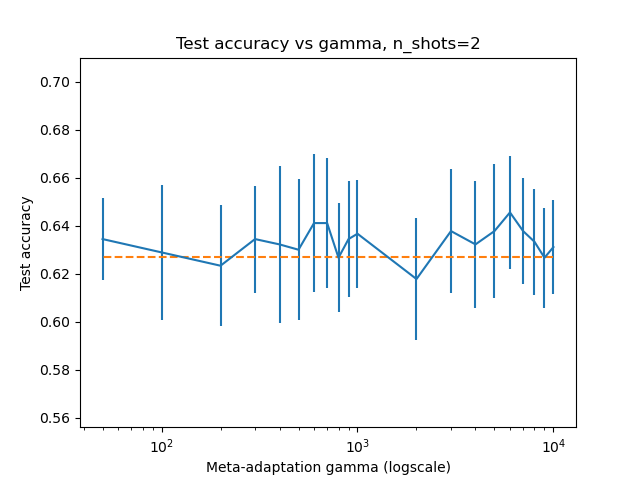
\includegraphics[width=\textwidth]{accuracy_plot_2}
		\caption{2-shot test adaptation}
	\end{subfigure}
	\hfill
	\begin{subfigure}[b]{0.49\textwidth}
		\centering
		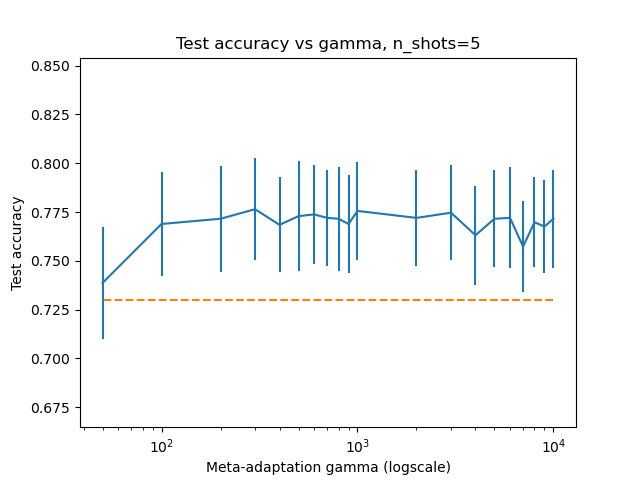
\includegraphics[width=\textwidth]{accuracy_plot_5}
		\caption{5-shot test adaptation}	 	
	\end{subfigure}
	\hfill
	\caption{Average test accuracies for meta-adaptation with different values of $\gamma$. All runs assumed $\beta\rightarrow\infty$. Error bars represent standard errors from the average over 10 runs.}	 
	\label{fig:results-gamma}
\end{figure}

\begin{table}	
	
	\centering
	\begin{tabular}{lll}
		\toprule
		Method   & Hyper-prior \#permuted pixels  & Test accuracy   \\
		\midrule
		Meta-testing, 2-shot & 100   & $0.777\pm 0.023 $      \\
		Adapted meta-testing, 2-shot & 100   & $0.672\pm ???$      \\
		\midrule
		Meta-testing, 2-shot & 1000   & $0.627\pm 0.025 $      \\
		Adapted meta-testing, 2-shot & 1000   & $0.646\pm 0.023$      \\
		\midrule
		Meta-testing, 5-shot & 100   & $0.86\pm 0.018$      \\
		Adapted meta-testing, 5-shot & 100   & $0.859\pm ???$      \\
		\midrule
		Meta-testing, 5-shot & 1000   & $0.73\pm 0.024$      \\
		Adapted meta-testing, 5-shot & 1000   & $0.776\pm 0.026$      \\
		\bottomrule
	\end{tabular}
	\caption{Best test accuracies for the permuted-MNIST dataset with variable hyper-priors and $\beta\rightarrow \infty$. All accuracies are averaged over 10 seeds and reported with standard error. Dashed line represents baseline meta-testing accuracy.}
	\label{table:gamma}
\end{table}

%TODO: explain findings

As we can see from Figure \ref{fig:results-gamma}, there is a noticeable improvement in accuracy for 


\LF{TODO: heatmap of beta/gamma vs accuracy. }

\section{Conclusions}

% Something

\clearpage
\bibliographystyle{plainnat}
\bibliography{library}

\section*{Checklist}

\begin{enumerate}
	
	\item For all authors...
	\begin{enumerate}
		\item Do the main claims made in the abstract and introduction accurately reflect the paper's contributions and scope?
		\answerTODO{}
		\item Did you describe the limitations of your work?
		\answerTODO{}
		\item Did you discuss any potential negative societal impacts of your work?
		\answerTODO{}
		\item Have you read the ethics review guidelines and ensured that your paper conforms to them?
		\answerTODO{}
	\end{enumerate}
	
	
	\item If you are including theoretical results...
	\begin{enumerate}
		\item Did you state the full set of assumptions of all theoretical results?
		\answerYes{}
		\item Did you include complete proofs of all theoretical results?
		\answerYes{}
	\end{enumerate}
	
	
	\item If you ran experiments...
	\begin{enumerate}
		\item Did you include the code, data, and instructions needed to reproduce the main experimental results (either in the supplemental material or as a URL)?
		\answerYes{}
		\item Did you specify all the training details (e.g., data splits, hyperparameters, how they were chosen)?
		\answerYes{}
		\item Did you report error bars (e.g., with respect to the random seed after running experiments multiple times)?
		\answerTODO{}
		\item Did you include the total amount of compute and the type of resources used (e.g., type of GPUs, internal cluster, or cloud provider)?
		\answerTODO{}
	\end{enumerate}
	
	
	\item If you are using existing assets (e.g., code, data, models) or curating/releasing new assets...
	\begin{enumerate}
		\item If your work uses existing assets, did you cite the creators?
		\answerYes{} Code and data, see citations (MAML, MNIST, SGLD, Adam, learn2learn)
		\item Did you mention the license of the assets?
		\answerTODO{}
		\item Did you include any new assets either in the supplemental material or as a URL?
		\answerYes{}
		\item Did you discuss whether and how consent was obtained from people whose data you're using/curating?
		\answerNA{} Standard datasets
		\item Did you discuss whether the data you are using/curating contains personally identifiable information or offensive content?
		\answerNA{} Standard datasets
	\end{enumerate}
	
	
	\item If you used crowdsourcing or conducted research with human subjects...
	\begin{enumerate}
		\item Did you include the full text of instructions given to participants and screenshots, if applicable?
		\answerNA{}
		\item Did you describe any potential participant risks, with links to Institutional Review Board (IRB) approvals, if applicable?
		\answerNA{}
		\item Did you include the estimated hourly wage paid to participants and the total amount spent on participant compensation?
		\answerNA{}
	\end{enumerate}
	
	
\end{enumerate}

\appendix
\section{Appendix}

\subsection{Hyper-parameters and implementation details} \label{append:hyper-params}

% TODO: hyper-params, quality of the prior, using adapt-eval split for less bias


Optionally include extra information (complete proofs, additional experiments and plots) in the appendix.
This section will often be part of the supplemental material.


\end{document}